% Exact Bayesian binning beyond one dimension -- draft.
%
% Every data-dependent number is a macro from data/numbers.tex, and every table body and plotted
% series is a file in data/, all written by the pipeline in scripts/ (see README.md and the
% Makefile). To update the paper with more data: `make data && make`. Claims in the text that the
% new results no longer support are listed in a box under the abstract (scripts/macros.py).

\documentclass[11pt,a4paper]{article}
\usepackage[T1]{fontenc}
\usepackage[utf8]{inputenc}
\usepackage{lmodern}
\usepackage[margin=2.4cm]{geometry}
\usepackage{amsmath,amssymb}
\usepackage{microtype}
\usepackage{graphicx}
\usepackage{booktabs}
\usepackage{xcolor}
\usepackage{tikz}
\usetikzlibrary{arrows.meta,positioning,calc}
\usepackage{pgfplots}
\pgfplotsset{compat=1.18}
\usepackage{pgfplotstable}
\usepackage[round]{natbib}
\usepackage[hidelinks]{hyperref}
\usepackage[capitalise,noabbrev]{cleveref}
\DeclareUnicodeCharacter{2265}{\ensuremath{\geq}}
% generated table rows: TeX's primitive \input is expandable, so \bottomrule may follow it
\makeatletter\newcommand{\rows}[1]{\@@input #1 }\makeatother

% Generated by scripts/macros.py from the pipeline's results; do not edit.
\newcommand{\allCells}{41,162}
\newcommand{\binaryPerPartition}{38}
\newcommand{\callOverhead}{0.5}
\newcommand{\checkEvidenceError}{2\times10^{-15}}
\newcommand{\checkPartitions}{5,832, 4,367, 2,500}
\newcommand{\checkRateError}{4\times10^{-14}}
\newcommand{\checkRecursiveError}{6\times10^{-15}}
\newcommand{\countBinaryTrees}{2,590,351}
\newcommand{\countGrid}{4\times4}
\newcommand{\countGuillotine}{68,480}
\newcommand{\countMultiwayTrees}{286,985}
\newcommand{\countProduct}{64}
\newcommand{\countSingles}{274}
\newcommand{\countTilings}{70,878}
\newcommand{\countTwoLevel}{5,832}
\newcommand{\finestRes}{3}
\newcommand{\multiwayPerPartition}{4.2}
\newcommand{\newsAlpha}{0.1}
\newcommand{\newsBestPerEvent}{$-0.017$}
\newcommand{\newsBinsResOne}{245}
\newcommand{\newsBinsResThree}{8,385}
\newcommand{\newsBinsResTwo}{997}
\newcommand{\newsBinsResZero}{41}
\newcommand{\newsCells}{4,008}
\newcommand{\newsDays}{4.5}
\newcommand{\newsEmptyBins}{6,009}
\newcommand{\newsEmptyChildren}{7,338}
\newcommand{\newsEmptyShare}{78\%}
\newcommand{\newsEvents}{127,367}
\newcommand{\newsFirst}{2026-09-26}
\newcommand{\newsGainGrid}{1,871}
\newcommand{\newsGainGridPerEvent}{0.024}
\newcommand{\newsGridTwoPerEvent}{$-1.18$}
\newcommand{\newsKansas}{2,643}
\newcommand{\newsLargestRegion}{397}
\newcommand{\newsLast}{2026-10-01}
\newcommand{\newsMerge}{1.4~s}
\newcommand{\newsMergedNoBonusPerEvent}{$-0.10$}
\newcommand{\newsMergedPerEvent}{$-0.11$}
\newcommand{\newsNodes}{5,882}
\newcommand{\newsPass}{0.8~ms}
\newcommand{\newsPriorMean}{10}
\newcommand{\newsRegions}{1,457}
\newcommand{\newsRho}{0.1}
\newcommand{\newsSearch}{0.27~s}
\newcommand{\newsShareResOne}{29\%}
\newcommand{\newsShareResThree}{20\%}
\newcommand{\newsShareResTwo}{17\%}
\newcommand{\newsShareResZero}{34\%}
\newcommand{\newsTestChange}{$+63$\%}
\newcommand{\newsTestDays}{2.2}
\newcommand{\newsTestEvents}{78,910}
\newcommand{\newsTrainDays}{2.2}
\newcommand{\newsTrainEvents}{48,457}
\newcommand{\newsTreeBins}{9,668}
\newcommand{\newsWorldPerEvent}{$-4.3$}
\newcommand{\oneDBayesbinSeconds}{2.1~s}
\newcommand{\oneDBinaryGain}{$+2.4$}
\newcommand{\oneDBinaryRho}{0.5}
\newcommand{\oneDBinarySeconds}{22~s}
\newcommand{\oneDDyadicLoss}{45}
\newcommand{\oneDDyadicSeconds}{11.0~ms}
\newcommand{\oneDEvents}{23,230}
\newcommand{\oneDMmap}{24}
\newcommand{\oneDT}{2,048}
\newcommand{\priorSettings}{336}
\newcommand{\quakeAlpha}{0.03}
\newcommand{\quakeBestPerEvent}{$-0.015$}
\newcommand{\quakeBinsResOne}{314}
\newcommand{\quakeBinsResThree}{4,354}
\newcommand{\quakeBinsResTwo}{1,288}
\newcommand{\quakeBinsResZero}{37}
\newcommand{\quakeCells}{1,708}
\newcommand{\quakeDays}{92.0}
\newcommand{\quakeEmptyBins}{4,615}
\newcommand{\quakeEmptyChildren}{4,945}
\newcommand{\quakeEmptyShare}{95\%}
\newcommand{\quakeEvents}{24,500}
\newcommand{\quakeFirst}{2026-06-27}
\newcommand{\quakeGainGrid}{777}
\newcommand{\quakeGainGridPerEvent}{0.066}
\newcommand{\quakeGridTwoPerEvent}{$-0.77$}
\newcommand{\quakeLargestRegion}{483}
\newcommand{\quakeLast}{2026-09-26}
\newcommand{\quakeMerge}{0.4~s}
\newcommand{\quakeMergedNoBonusPerEvent}{$-0.24$}
\newcommand{\quakeMergedPerEvent}{$-0.26$}
\newcommand{\quakeNodes}{2,799}
\newcommand{\quakePass}{0.5~ms}
\newcommand{\quakePriorMean}{10}
\newcommand{\quakeRegions}{539}
\newcommand{\quakeRho}{0.1}
\newcommand{\quakeSearch}{0.18~s}
\newcommand{\quakeShareResOne}{37\%}
\newcommand{\quakeShareResThree}{11\%}
\newcommand{\quakeShareResTwo}{22\%}
\newcommand{\quakeShareResZero}{30\%}
\newcommand{\quakeTestChange}{$-7$\%}
\newcommand{\quakeTestDays}{46.0}
\newcommand{\quakeTestEvents}{11,777}
\newcommand{\quakeTrainDays}{46.0}
\newcommand{\quakeTrainEvents}{12,723}
\newcommand{\quakeTreeBins}{5,993}
\newcommand{\quakeWorldPerEvent}{$-5.1$}
\newcommand{\recursiveHundred}{17~s}
\newcommand{\recursiveMBHundred}{204}
\newcommand{\recursiveMBSixtyFour}{35}
\newcommand{\recursiveMBThirtyTwo}{2}
\newcommand{\recursiveSixtyFour}{2~s}
\newcommand{\recursiveThirtyTwo}{84.5~ms}
\newcommand{\streamAlarmsAlone}{44}
\newcommand{\streamAlarmsResTwo}{70}
\newcommand{\streamAlarmsTree}{56}
\newcommand{\streamBigAlone}{329}
\newcommand{\streamBigAlonePct}{58\%}
\newcommand{\streamBigQuakes}{571}
\newcommand{\streamBigResTwo}{463}
\newcommand{\streamBigResTwoPct}{81\%}
\newcommand{\streamBigTree}{409}
\newcommand{\streamBigTreeAll}{468}
\newcommand{\streamBigTreeAllPct}{82\%}
\newcommand{\streamBigTreePct}{72\%}
\newcommand{\streamBusyCells}{15}
\newcommand{\streamBusyResTwoLoss}{4.6}
\newcommand{\streamBusySelf}{98\%}
\newcommand{\streamBusyTailAlone}{1.19}
\newcommand{\streamBusyTailResTwo}{4.75}
\newcommand{\streamBusyTailTree}{1.22}
\newcommand{\streamCells}{1,708}
\newcommand{\streamDays}{90}
\newcommand{\streamEvents}{24,500}
\newcommand{\streamGain}{12,448}
\newcommand{\streamGainAll}{9,539}
\newcommand{\streamGainMonth}{10,279}
\newcommand{\streamGainResTwo}{1,338}
\newcommand{\streamMediumCells}{118}
\newcommand{\streamMediumSelf}{79\%}
\newcommand{\streamMediumTailAlone}{0.91}
\newcommand{\streamMediumTailResTwo}{1.62}
\newcommand{\streamMediumTailTree}{1.07}
\newcommand{\streamRareBase}{59\%}
\newcommand{\streamRareCells}{1,061}
\newcommand{\streamRareSelf}{2\%}
\newcommand{\streamRareTailAlone}{0.44}
\newcommand{\streamRareTailResTwo}{0.90}
\newcommand{\streamRareTailTree}{0.99}
\newcommand{\streamRho}{0.1}
\newcommand{\streamSparseCells}{514}
\newcommand{\streamSparseSelf}{13\%}
\newcommand{\streamSparseTailAlone}{0.51}
\newcommand{\streamSparseTailResTwo}{0.95}
\newcommand{\streamSparseTailTree}{1.02}
\newcommand{\streamWindowMinutes}{5}
\newcommand{\streamWindows}{25,919}
\newcommand{\twoLevelEvidenceHundred}{5.1~s}
\newcommand{\twoLevelEvidenceOneTwentyEight}{9.9~s}
\newcommand{\twoLevelEvidenceSixtyFour}{1.8~s}
\newcommand{\twoLevelEvidenceThirtyTwo}{0.4~s}
\newcommand{\twoLevelEvidenceTwoHundred}{44~s}
\newcommand{\twoLevelMHundred}{7}
\newcommand{\twoLevelMOneTwentyEight}{9}
\newcommand{\twoLevelMSixtyFour}{7}
\newcommand{\twoLevelMThirtyTwo}{4}
\newcommand{\twoLevelMTwoHundred}{10}
\newcommand{\twoLevelRatesHundred}{2.5~s}
\newcommand{\twoLevelRatesOneTwentyEight}{2.8~s}
\newcommand{\twoLevelRatesSixtyFour}{1.1~s}
\newcommand{\twoLevelRatesThirtyTwo}{0.41~s}
\newcommand{\twoLevelRatesTwoHundred}{2.3~s}
\newcommand{\claimwarnings}{}
\newcommand{\claimcount}{0}


\definecolor{binfill}{HTML}{CDE2FB}
\definecolor{binline}{HTML}{1C5CAB}
\definecolor{accent}{HTML}{EB6834}
\newcommand{\R}{\mathbb{R}}
\newcommand{\E}{\mathbb{E}}
\newcommand{\km}{\,km\textsuperscript{2}}

\title{Exact Bayesian binning beyond one dimension:\\chains, trees and the globe\\[0.4em]
  \large Draft, \today}
\author{Peter F\"oldi\'ak\thanks{Affiliation and contact to be added.}}
\date{}

\begin{document}
\maketitle

\begin{abstract}
Bayesian binning models a rate along an ordered axis as piecewise constant and sums exactly
over every segmentation and every number of bins by dynamic programming. We ask which families of
two-dimensional partitions keep that exactness. The sum stays exact and polynomial whenever the
partitions are built by nesting chains and trees: rows into bands with each band's own columns, at
$O(M N^2)$ for $N$ cells; recursive cuts, at $O(N^2(m+n))$ for an $m \times n$ grid; and any fixed
hierarchy of regions, such as the H3 cells of the globe, in time linear in the number of nodes. It
does not stay exact for product grids, general tilings or polygons, for which even the single best
partition is NP-hard to find. Over the H3 tree of the globe, one pass bins \newsEvents\ news events
in \newsPass, with the prior chosen by the evidence: empty ocean gets bins of four million
square kilometres and every city the finest cells the data have. Fitted on the first half of each
record, the posterior average over the tree's partitions predicts the second half better than every
fixed grid, for news events and for earthquakes; greedy merging of neighbouring bins gives cleaner
maps but predicts worse. In one dimension a hierarchical prior adds nothing: a binary-cut tree ties
with the original prior at many times the cost, and a dyadic tree loses. Nesting stays quadratic in
the number of cells in any dimension, which makes space--time binning exact.
\end{abstract}

\ifnum\claimcount>0
\begin{center}
\fcolorbox{accent}{accent!6}{\parbox{0.92\linewidth}{\small\textbf{After the last rerun, these
claims in the text need revisiting} (from \texttt{scripts/macros.py}):
\begin{itemize}\claimwarnings\end{itemize}}}
\end{center}
\fi

% ----------------------------------------------------------------------------------------------
\section{Introduction}

A rate that varies along one axis, observed as counts in intervals, is the setting of
peri-stimulus time histograms, event counts per window and change points. Bayesian binning
\citep{endres2008bayesian} treats the rate as piecewise constant with an unknown number of bins at
unknown positions, gives each bin a conjugate prior, and sums the posterior exactly over every
segmentation by dynamic programming. It needs no bin width, gives error bars and a posterior over
the number of bins, and on real spike trains it predicted held-out data better than fixed-width
histograms and kernels \citep{endres2008bayesian}.

Many rates vary over a plane, or over the surface of the Earth, as well as in time. A system that
watches the world's open data streams for anomalies, such as the Worldwatch project that motivates
this note, counts events per cell of a global hexagonal grid \citep{h3} at a resolution fixed per
stream. A fixed resolution pools too little where data are sparse and too much where they are
dense. The one-dimensional method resolves each stretch at the scale its data support; we ask
whether that carries over to two dimensions, at what cost, and whether the resulting bins predict
better.

The dynamic programme relies on the order of the axis, and a plane has none. What it really
needs, however, is a way of building partitions from sub-problems that meet only at their own
boundaries. \Cref{sec:needs} makes this precise and sorts the natural families of 2-D partitions
into those that keep an exact sum (\cref{sec:exact}) and those that do not (\cref{sec:notexact}).
\Cref{sec:experiments} measures the exact ones: their cost on grids, a binning of the globe from
Worldwatch's news-event and earthquake counts, held-out prediction against fixed grids, and
whether a hierarchy would help in one dimension. \Cref{sec:higher} sketches three and more
dimensions.

% ----------------------------------------------------------------------------------------------
\section{Bayesian binning in one dimension}\label{sec:oned}

The axis has $T$ intervals; interval $k$ has a count $y_k$ and an exposure $e_k$ (time, area,
population). A partition into $M+1$ contiguous bins gives each bin $B$ a rate $\lambda_B$ with a
Gamma$(\alpha, \beta)$ prior. Given the partition the counts are Poisson, and each bin's rate
integrates out to its evidence
\begin{equation}
  L(B) = \frac{\beta^\alpha}{\Gamma(\alpha)}\,
         \frac{\Gamma(\alpha + Y_B)}{(\beta + E_B)^{\alpha + Y_B}},
  \qquad Y_B = \sum_{k \in B} y_k,\quad E_B = \sum_{k \in B} e_k,
  \label{eq:bin}
\end{equation}
up to a factor $\prod_k e_k^{y_k} / y_k!$ that is the same for every partition. (A Bernoulli
model with a Beta prior works the same way.) The prior on partitions is uniform on $M \in
\{0, \dots, M_{\max}\}$ and uniform over the $\binom{T-1}{M}$ boundary positions given $M$. The
evidence of $M$ is a sum over all segmentations, computed by the forward recursion
\begin{equation}
  f_m(k) = \sum_{j \le k} f_{m-1}(j-1)\, L(j, k), \qquad f_0(k) = L(1, k),
  \label{eq:forward}
\end{equation}
where $f_m(k)$ is the evidence of intervals $1..k$ as $m+1$ bins. A matching backward recursion
gives the posterior probability of every candidate bin, hence the predictive rate, its standard
deviation and the posterior of a boundary after each interval, averaged over all $M$. The cost is
$O(M T^2)$ time and, computing bin evidences on the fly from prefix sums, $O(MT)$ memory
\citep{bayesbin}.

What makes \cref{eq:forward} possible is that the rest of a partition meets ``intervals $1..k$''
only at $k$: one number summarises everything to the left.

% ----------------------------------------------------------------------------------------------
\section{What the dynamic programme needs}\label{sec:needs}

The exact sum needs three things, and an ordered axis gives all three:
(i) polynomially many candidate bins, here the $T(T+1)/2$ intervals;
(ii) each bin's evidence in $O(1)$, here from prefix sums; and
(iii) partitions that break into sub-problems meeting the rest only at their own boundary.

Take an $m \times n$ grid of cells, $N = mn$, with a count and an exposure per cell. Condition
(ii) still holds for rectangles: a rectangle's totals are four lookups in a summed-area table, and
\cref{eq:bin} applies to them. What decides each family of 2-D partitions is condition (iii).
Families built by nesting chains and trees keep it, because their sub-problems are intervals,
rectangles (four numbers, about $N^2/4$ of them) or the nodes of a fixed hierarchy; the sums are
then inside passes in the sense of context-free parsing \citep{younger1967recognition,lari1990estimation}.
Families defined by one choice shared across the grid, or by free adjacency, lose it.
\Cref{fig:families} shows the rectangle families, and \cref{tab:families} summarises all of them.

\begin{figure}[t]
\centering
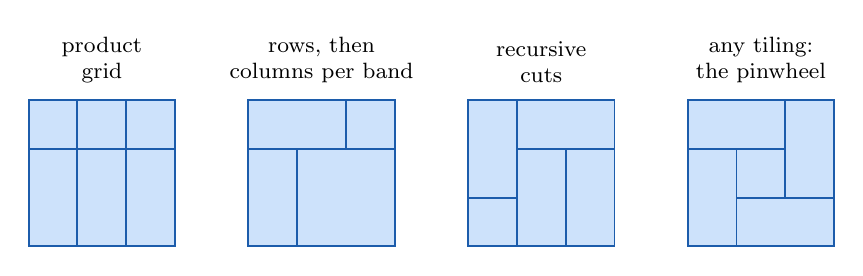
\begin{tikzpicture}[x=0.62cm,y=0.62cm, bin/.style={fill=binfill, draw=binline, line width=0.6pt}]
  \newcommand{\panel}[3]{% x offset, title line 1, title line 2
    \begin{scope}[shift={(#1,0)}]
      \fill[binfill] (0,0) rectangle (3,3);
      \node[font=\footnotesize, align=center, anchor=south] at (1.5,3.15) {#2\\#3};
    \end{scope}}
  \panel{0}{product}{grid}
  \panel{4.5}{rows, then}{columns per band}
  \panel{9}{recursive}{cuts}
  \panel{13.5}{any tiling:}{the pinwheel}
  \begin{scope}[draw=binline, line width=0.7pt]
    % product grid: one row cut, two column cuts
    \draw (0,0) rectangle (3,3); \draw (0,2) -- (3,2); \draw (1,0) -- (1,3); \draw (2,0) -- (2,3);
    % rows, then columns per band
    \draw (4.5,0) rectangle (7.5,3); \draw (4.5,2) -- (7.5,2); \draw (6.5,2) -- (6.5,3); \draw (5.5,0) -- (5.5,2);
    % recursive cuts: depth three
    \draw (9,0) rectangle (12,3); \draw (10,0) -- (10,3); \draw (9,1) -- (10,1); \draw (10,2) -- (12,2); \draw (11,0) -- (11,2);
    % pinwheel: no straight line through the whole
    \draw (13.5,0) rectangle (16.5,3); \draw (13.5,2) -- (15.5,2); \draw (15.5,1) -- (15.5,3);
    \draw (14.5,1) -- (16.5,1); \draw (14.5,0) -- (14.5,2);
  \end{scope}
\end{tikzpicture}
\caption{Families of rectangle partitions, each strictly inside the next: product grids,
rows then columns per band, recursive (guillotine) cuts, and all tilings. The pinwheel is the
smallest tiling that no sequence of straight cuts produces. On a $\countGrid$ grid there are
\countTilings\ tilings, of which \countGuillotine\ are guillotine, \countTwoLevel\ are rows then
columns and \countProduct\ are product grids.}
\label{fig:families}
\end{figure}

\begin{table}[t]
\centering\small
\begin{tabular}{@{}p{0.27\linewidth}p{0.17\linewidth}p{0.21\linewidth}p{0.1\linewidth}p{0.14\linewidth}@{}}
\toprule
family & exact sum & cost (time; memory) & each partition once & $P(M \mid D)$ \\
\midrule
product grid (shared cuts) & no; yes if one axis is short & Gibbs sampling & yes & estimated \\
rows, then columns per band & yes & $O(MN^2)$; $O(m^2 + Mn)$ & yes & per level \\
recursive cuts (guillotine) & yes & $O(N^2(m+n))$; $O(N^2)$ & no & per-split prior \\
any rectangular tiling & no (\#P-hard) & MCMC & -- & estimated \\
polygons, regions on a map & no & MCMC & -- & estimated \\
cells along a Hilbert curve & yes & $O(MN^2)$; $O(MN)$ & yes & yes \\
a fixed hierarchy (H3) & yes & $O(\text{nodes})$ & yes & per-split prior \\
\bottomrule
\end{tabular}
\caption{Families of 2-D partitions and what each keeps of the 1-D method. The rate and its error
bars per cell are exact wherever the sum is.}
\label{tab:families}
\end{table}

% ----------------------------------------------------------------------------------------------
\section{Exact families}\label{sec:exact}

\subsection{Rows, then each band its own columns}\label{sec:twolevel}

Choose row cuts $R$ with the 1-D prior; then each band $b$, independently, chooses its own column
cuts $C_b$ with the same prior. The bins are the rectangles band $\times$ column interval, and
\begin{equation}
  Z = \sum_R P(R) \prod_{\text{bands } b} Z_b, \qquad
  Z_b = \sum_{C_b} P(C_b) \prod_{c} L(b \times c).
  \label{eq:twolevel}
\end{equation}
$Z_b$ is the 1-D marginal likelihood of the band's column series, its counts and exposures summed
over the band's rows, so the whole computation is the 1-D method twice. For each of the
$m(m+1)/2$ candidate bands, the forward recursion on its column series gives $\log Z_b$; these form
a table of bin evidences over the rows, on which the 1-D forward and backward recursions give the
evidence of every number of row cuts and the posterior $W_{ab}$ that rows $a..b$ form a band. The
rate and second moment at cell $(i,j)$ are $\sum_{a \le i \le b} W_{ab}$ times band $[a,b]$'s values
at column $j$, from the bands' own backward passes.

Everything the 1-D method has survives. Each partition arises once, since the bands are the
distinct top and bottom edges of its rectangles, so the prior is the 1-D one at both levels; there
are $2^{n-1}(1 + 2^{n-1})^{m-1}$ such partitions. The posterior over the number of row cuts is
exact, and so is that over each band's number of column cuts. The cost is $O(M m^2 n^2) = O(MN^2)$,
quadratic in the number of cells as the 1-D method is in $T$, with $O(m^2 + Mn)$ memory. One
practical point: the data-only factor of a band's summed series differs from band to band, so it
must be left out of $Z_b$ and the grid's own factor added once.

What is lost is symmetry: rows-first and columns-first are different priors. Their equal mixture
is still exact, at twice the cost, and its posterior weights say which orientation the data
prefer. The outer axis need not be ordered either: the seven days of a week can be grouped by any
set partition, each group with its own time-of-day profile, in 127 fits and an exact sum over 877
groupings.

\subsection{Recursive cuts}\label{sec:guillotine}

Let each rectangle be one bin with probability $\rho$, or be cut straight through, horizontally or
vertically (half each where both are possible), at a uniform position, each part being binned the
same way. The evidence is an inside pass over all sub-rectangles in order of size: for an $h \times
w$ rectangle $R$,
\begin{equation}
  Z(R) = \rho L(R) + (1-\rho)\Bigl[\tfrac{1}{2(h-1)} \sum_{k} Z(R^{\uparrow}_k) Z(R^{\downarrow}_k)
        + \tfrac{1}{2(w-1)} \sum_{k} Z(R^{\leftarrow}_k) Z(R^{\rightarrow}_k)\Bigr],
  \label{eq:guillotine}
\end{equation}
with $Z = L$ for a single cell and weight one for a direction that is the only one possible. An
outside pass of the same cost gives every sub-rectangle's posterior probability of being a bin.
There are about $N^2/4$ sub-rectangles with $h + w - 2$ cuts each, $m^2n^2(m+n)/12$ terms in all;
the table of inside values takes $N^2/4$ numbers, and memory is the practical limit.

Two properties of the 1-D method are lost. A partition with crossing cuts comes from several
construction trees: on a $\countGrid$ grid, the \countGuillotine\ guillotine partitions come from
\countBinaryTrees\ binary cut trees, \binaryPerPartition\ per partition on average. Letting a node
take all its parallel cuts at once, as the 1-D step chooses a set of boundaries, removes the
duplicates of associativity and leaves \countMultiwayTrees\ trees, \multiwayPerPartition\ per
partition; the partition into single cells still arises \countSingles\ times. Counting each
partition once would need a constraint across siblings that the recursion cannot see, so the prior
is over construction trees, as in Bayesian CART \citep{chipman1998bayesian,denison1998bayesian}
and the Mondrian process \citep{roy2008mondrian}. And tracking the number of bins would cost a
convolution at every cut, so a per-split probability replaces the uniform prior on $M$. Restricting
cuts to dyadic positions leaves $O(N)$ sub-problems, as in optional P\'olya trees
\citep{wong2010optional} and in the search for the best dyadic partition
\citep{donoho1997cart,kolaczyk2004multiscale,willett2007multiscale}, at the price of fixed boundary
positions.

\begin{table}[t]
\centering\small
\begin{tabular}{@{}lrrrrrr@{}}
\toprule
grid & tilings & guillotine & rows, then columns & product grids & binary cut trees & multi-way cut trees \\
\midrule
\rows{data/counts_table.tex}
\bottomrule
\end{tabular}
\caption{Partitions of small grids by family, and the construction trees of the recursive-cut
prior. Multi-way trees take all of a node's parallel cuts at once.}
\label{tab:counts}
\end{table}

\subsection{Fixed hierarchies and the globe}\label{sec:tree}

A fixed hierarchy of regions, such as a quadtree, administrative areas or the H3 cells of the
globe, gives an exact recursion from the leaves: each node $\nu$ is one bin, or its children are
binned the same way,
\begin{equation}
  Z(\nu) = \rho\, L(\nu) + (1-\rho) \prod_{\chi \in \text{children}(\nu)} Z(\chi),
  \qquad Z = L \text{ at the finest level}.
  \label{eq:tree}
\end{equation}
The cost is linear in the number of nodes, and each partition, a pruned subtree, arises once.
Working down from the root, $P(\nu \text{ reached} \mid D) = P(\pi \text{ reached} \mid D)\,
(1-\rho) \prod_{\chi} Z(\chi) / Z(\pi)$ for the parent $\pi$ of $\nu$, and $P(\nu \text{ is a bin}
\mid D) = P(\nu \text{ reached} \mid D)\, \rho L(\nu) / Z(\nu)$; the posterior mean rate of a cell
averages its ancestors' rates under these probabilities.

H3 is such a tree \citep{h3}: twelve pentagons and otherwise hexagons at every resolution, each cell
with seven children (six for a pentagon). A child hexagon is not inside its parent's, but every
finest cell has one ancestor at each resolution, so the finest descendants of the cells of any
resolution partition the finest cells exactly; a node's region is the set of its finest
descendants. We add a root, the whole world, above the 122 base cells. A child with no events
below it is taken as a single empty bin, since an empty region has nothing to split on; this keeps
the cost proportional to the nodes with data. Two limits follow from the fixed tree. Bins follow
the hierarchy's boundaries, so a hotspot on a parent's edge splits both parents, and when a cell
splits all seven children become bins. Letting a node group its children (each group of two or
more one bin, each child left alone binned recursively) relieves both and stays exact, at a sum
over the 877 groupings of seven children per node.

\begin{figure}[t]
\centering
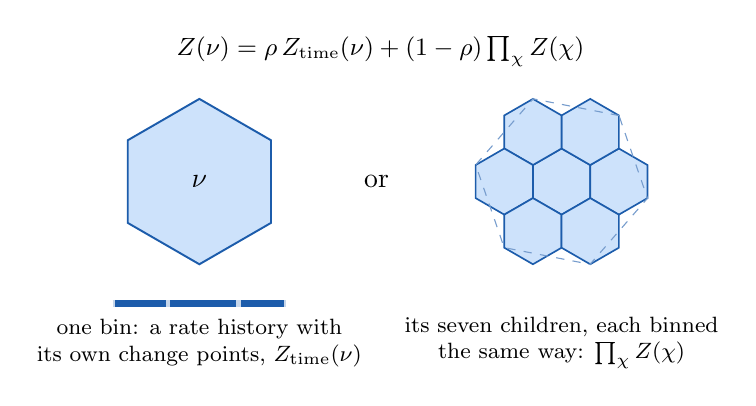
\begin{tikzpicture}[x=1cm,y=1cm]
  \newcommand{\hexagon}[3]{% centre, circumradius, style
    \draw[#3] ($(#1)+(30:#2)$) -- ($(#1)+(90:#2)$) -- ($(#1)+(150:#2)$) -- ($(#1)+(210:#2)$)
      -- ($(#1)+(270:#2)$) -- ($(#1)+(330:#2)$) -- cycle;}
  % one bin: the region with its own change points in time
  \hexagon{0,0}{1.05}{fill=binfill, draw=binline, line width=0.7pt}
  \node at (0,0) {$\nu$};
  \draw[line width=2.6pt, binline!25] (-1.1,-1.55) -- (1.1,-1.55);
  \foreach \x/\w in {-1.1/0.7, -0.4/0.9, 0.5/0.6} \draw[line width=2.6pt, binline] (\x+0.03,-1.55) -- (\x+\w-0.03,-1.55);
  \node[font=\footnotesize, align=center] at (0,-2.05) {one bin: a rate history with\\its own change points, $Z_{\text{time}}(\nu)$};
  \node at (2.25,0) {or};
  % its seven children, each binned the same way
  \begin{scope}[shift={(4.6,0)}]
    \def\hexr{0.42}
    \hexagon{0,0}{\hexr}{fill=binfill, draw=binline, line width=0.6pt}
    \foreach \a in {0,60,...,300} {\hexagon{\a:{sqrt(3)*\hexr}}{\hexr}{fill=binfill, draw=binline, line width=0.6pt}}
    \draw[dashed, binline!60] (49:{sqrt(7)*\hexr}) \foreach \a in {109,169,...,409} { -- (\a:{sqrt(7)*\hexr})} -- cycle;
    \node[font=\footnotesize, align=center] at (0,-2.05) {its seven children, each binned\\the same way: $\prod_{\chi} Z(\chi)$};
  \end{scope}
  \node[font=\small] at (2.3,1.65) {$Z(\nu) = \rho\, Z_{\text{time}}(\nu) + (1-\rho) \prod_{\chi} Z(\chi)$};
\end{tikzpicture}
\caption{The recursion over the H3 tree, with time nested inside each node
(\cref{sec:spacetime}). A region is either one bin with its own segmentation in time, or its
children differ. The dashed outline is the parent hexagon, which its children do not exactly
fill.}
\label{fig:tree}
\end{figure}

\subsection{Time inside space}\label{sec:spacetime}

Nesting works across kinds of axis as well. Replacing $L(\nu)$ in \cref{eq:tree} by
$Z_{\text{time}}(\nu)$, the 1-D marginal likelihood of the region's summed counts over time, makes
each region either one rate history with its own change points, or lets its children differ
(\cref{fig:tree}). This is exact at one 1-D model per node, and it streams: Bayesian online
change-point detection \citep{adams2007bayesian,fearnhead2007online} per node keeps that node's
running evidence, the recursion costs $O(\text{nodes})$ per window, and a cell's predictive for
the next window is the mixture of its ancestors' predictives weighted by the probability that
each is the cell's bin given the data so far. The pooling is then the same for all time, so a
burst in one cell separates it from its neighbours for its whole history.

Both limits go if the sub-problems are blocks: a region $\nu$ over an interval $a..b$ of time is one
bin, or is cut in time at some $k$, or is split into $\nu$'s children over $a..b$,
\begin{equation}
  Z(\nu, a, b) = \rho\, L(\nu, a, b) + (1-\rho)\Bigl[\tfrac{\tau}{b-a}\sum_{k} Z(\nu, a, k)\, Z(\nu, k+1, b)
                 + (1-\tau) \prod_{\chi} Z(\chi, a, b)\Bigr],
  \label{eq:blocks}
\end{equation}
which is exact at $O(\text{nodes} \cdot T^3)$ time and $O(\text{nodes} \cdot T^2)$ memory. Each place
can then pool differently in different epochs, and each region has its own change points. Putting
space inside time instead (epochs with their own map) is also exact, but every local burst then
needs a new global epoch.

% ----------------------------------------------------------------------------------------------
\section{Families that are not exact}\label{sec:notexact}

\paragraph{Product grids.} With row cuts $R$ and column cuts $C$ each chosen once for the whole
grid, $Z = \sum_R \sum_C P(R) P(C) \prod_{r} \prod_{c} L(r \times c)$. Given $C$, a band's factor
depends only on its two boundaries, so the 1-D recursion over rows is exact, and likewise over
columns given $R$. But $C$ is shared by every band: a recursion down the rows would have to carry
the whole column partition as its state, $2^{n-1}$ values. No polynomial method is known, and even
the single best $p \times q$ grid is NP-complete to find for a sum of squared deviations
\citep{muthukrishnan2005approximation}, an additive objective like a sum of log evidences; see
also \citet{grigni1996complexity}. Product grids are a small subset of the previous family, yet
harder: a choice shared across the grid couples pieces that were otherwise independent. What
survives is exact conditionals, so blocked Gibbs sampling draws all row cuts given the columns and
then all column cuts given the rows, and the rate can be Rao-Blackwellised; the evidence can be
estimated from the exact conditionals \citep{chib1995marginal}. With one short axis, every
partition of it can be enumerated instead.

\paragraph{General tilings.} No recursion builds the pinwheel of \cref{fig:families}, and a sweep
across the grid would have to carry its whole frontier. With arbitrary weights per rectangle the
sum includes counting the monomer--dimer covers of a region of the grid, which is \#P-complete
\citep{jerrum1987two}, and the single best tiling is NP-hard \citep{muthukrishnan1999rectangular}.
General tilings also buy little: a tiling into $k$ rectangles has a guillotine refinement into at
most $2k - 1$ \citep{berman2002exact}, and in binning a refinement costs only an Occam factor,
since the rates on either side of an extra cut can be equal.

\paragraph{Polygons and regions on a map.} Voronoi tessellations around free generator points
\citep{byers2002bayesian}, connected groups of the regions of a map \citep{knorrheld2000bayesian}
and pieces of random spanning trees \citep{teixeira2019bayesian} need reversible-jump or other
MCMC \citep{green1995reversible}; Bayesian Blocks' route to higher dimensions merges neighbouring
Voronoi cells of the events \citep{scargle2001bayesian}. Conjugacy survives, so each bin's rate is
integrated out, but the exact evidence, the posterior of every candidate bin and the error bounds
are lost. Polygons buy less than they seem: the posterior mean over many rectangle partitions
already has contours that follow the data, as the 1-D average smooths a step.

\paragraph{Rescuing the order.} Numbering the cells along a Hilbert curve \citep{hilbert1891stetige}
and binning in 1-D is exact at $O(MN^2)$, and every quadtree partition is among its segmentations.
Its bins are runs of the curve, connected and compact but ragged, and the prior depends on where
the curve runs.

% ----------------------------------------------------------------------------------------------
\section{Experiments}\label{sec:experiments}

\subsection{Exactness and cost on rectangle grids}

Both exact rectangle families were implemented on Poisson counts with a Gamma$(1,1)$ prior per bin:
rows then columns per band with the bayesbin package \citep{bayesbin} doing every 1-D pass, and
recursive cuts as a numba kernel. Rows then columns agreed with enumeration of every partition
(\checkPartitions\ partitions on $4 \times 4$, $4 \times 5$ and $5 \times 4$ grids) to
$\checkEvidenceError$ in $\log P(D)$ and $\checkRateError$ in every cell's rate; recursive cuts
agreed with an independent memoised recursion to $\checkRecursiveError$. \Cref{fig:timings} shows
the cost on square grids with a planted disc and rectangle, on a four-core laptop. Rows then
columns took \twoLevelEvidenceHundred\ for the evidence of a $100 \times 100$ grid and
\twoLevelEvidenceTwoHundred\ at $200 \times 200$; about \callOverhead~ms of each band is the call
into the 1-D code, most of the time at these sizes. Recursive cuts took \recursiveHundred\ at $100
\times 100$, with a \recursiveMBHundred~MB table. The most probable number of row cuts grew with
the resolution (\twoLevelMThirtyTwo\ at $32 \times 32$, \twoLevelMHundred\ at $100 \times 100$),
because rectangles draw the disc's curved edge as a staircase.

\begin{figure}[t]
\centering
\begin{tikzpicture}
\begin{loglogaxis}[width=0.55\linewidth, height=5.2cm, xlabel={grid side ($m = n$)}, ylabel={seconds},
    xtick={32,64,100,128,200}, xticklabels={32,64,100,128,200},
    legend style={font=\footnotesize, draw=none, fill=none, at={(1.03,0.5)}, anchor=west, cells={anchor=west}}, tick label style={font=\footnotesize},
    label style={font=\small}, grid=major, grid style={gray!20}]
  \addplot[binline, mark=*, mark size=1.6pt, thick] table[col sep=comma, x=side, y=seconds] {data/plot_two_level_evidence.csv};
  \addlegendentry{rows then columns: evidence}
  \addplot[binline!55, mark=o, mark size=1.6pt, thick] table[col sep=comma, x=side, y=seconds] {data/plot_two_level_rates.csv};
  \addlegendentry{rows then columns: rates}
  \addplot[accent, mark=square*, mark size=1.6pt, thick] table[col sep=comma, x=side, y=seconds] {data/plot_recursive_evidence.csv};
  \addlegendentry{recursive cuts: evidence}
\end{loglogaxis}
\end{tikzpicture}
\caption{Time on square grids (four cores). The rates of rows then columns refit only the bands
with posterior probability above $10^{-12}$.}
\label{fig:timings}
\end{figure}

\subsection{Binning the globe}

The data are two of Worldwatch's streams, counted per H3 resolution-\finestRes\ cell (about
12,000\km, 110~km across; \allCells\ cells): \newsEvents\ news events from GDELT
\citep{leetaru2013gdelt} over \newsDays\ days (\newsFirst\ to \newsLast), in \newsCells\ cells, and
\quakeEvents\ earthquakes of magnitude at least 1 from the USGS catalogue \citep{usgs-comcat} over
\quakeDays\ days (\quakeFirst\ to \quakeLast), in \quakeCells\ cells. The exposure is area times
days. The prior's shape, mean and split probability were chosen by the evidence over
\priorSettings\ settings: $\alpha = \newsAlpha$ for news and $\quakeAlpha$ for earthquakes, a prior
mean \newsPriorMean\ times the global rate, $\rho = \newsRho$. One pass over the \newsNodes\ nodes
of the news tree took \newsPass\ and the whole search \newsSearch.

\Cref{fig:bins} shows the best partition (the maximum of \cref{eq:tree}). For news it has
\newsTreeBins\ bins: \newsBinsResZero\ resolution-0 bins over empty ocean, the Sahara and Siberia
covering \newsShareResZero\ of the Earth, and \newsBinsResThree\ of the finest cells wherever there
are events (\cref{tab:places}). For earthquakes the \quakeTreeBins\ bins follow the plate boundaries
and the dense US networks. Greedy merging of neighbouring bins while the evidence rises (with a
bonus of $\log 10$ per merge) leaves \newsRegions\ and \quakeRegions\ regions; the empty space then
becomes one connected region, and empty regions cover \newsEmptyShare\ and \quakeEmptyShare\ of the
Earth. \Cref{fig:zoom} shows the halos of empty sibling bins that the seven-way split leaves around
hotspots, which merging removes, and \cref{fig:rates} the posterior mean rates.

The bins shrink where the rate changes and there are enough events to show it, not where events are
numerous as such: a uniformly busy area would stay one bin. They also follow how the events are
observed. GDELT places stories it can only place by country at that country's centre, so the cell
at the centre of the contiguous US holds \newsKansas\ news events; the USGS records small
earthquakes densely only near US networks. And the exposure decides what counts as normal: with
area, bins split where events per square kilometre change; with population they would split where
events per person change.

\begin{figure}[t]
\centering
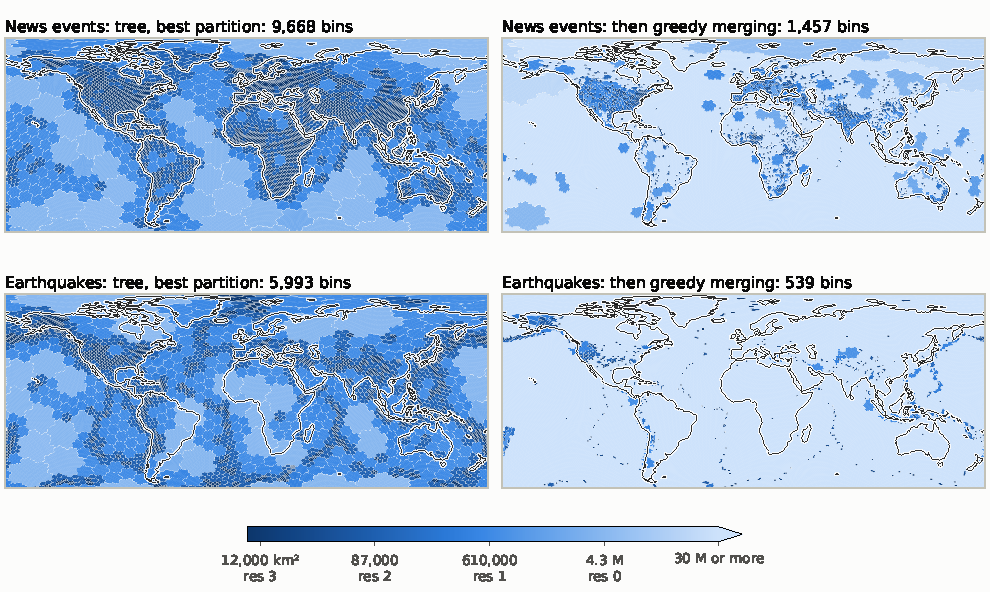
\includegraphics[width=\linewidth]{figures/globe_bins.pdf}
\caption{Bin sizes of the best partition over the H3 tree (left) and after greedy merging of
neighbouring bins (right), for news events (top) and earthquakes (bottom). Lighter is larger;
white lines are bin boundaries. Coastlines from \citet{naturalearth}.}
\label{fig:bins}
\end{figure}

\begin{figure}[t]
\centering
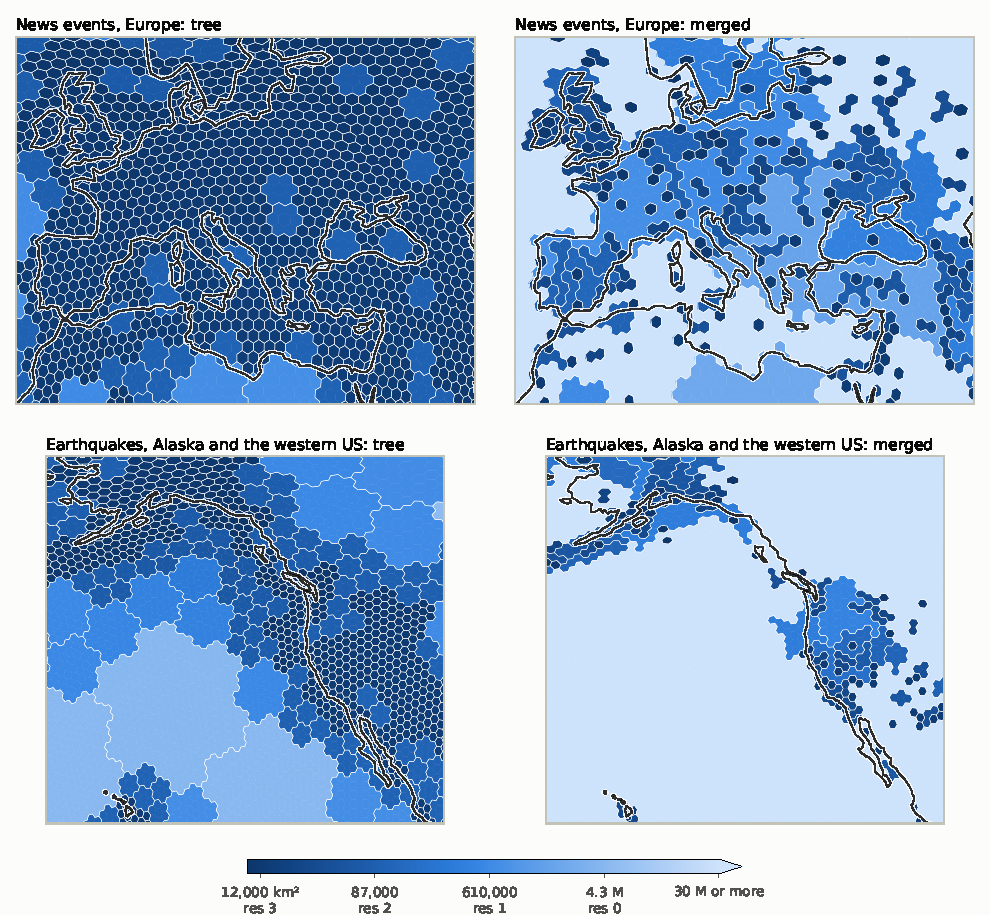
\includegraphics[width=0.92\linewidth]{figures/globe_zoom.pdf}
\caption{Close-ups of \cref{fig:bins}. In the tree's best partition a split turns all seven
children into bins, so fine bins spread over the Mediterranean next to coastal cities; merging
removes these halos, keeps the cities small and pools the countryside into regions of similar
rate.}
\label{fig:zoom}
\end{figure}

\begin{figure}[t]
\centering
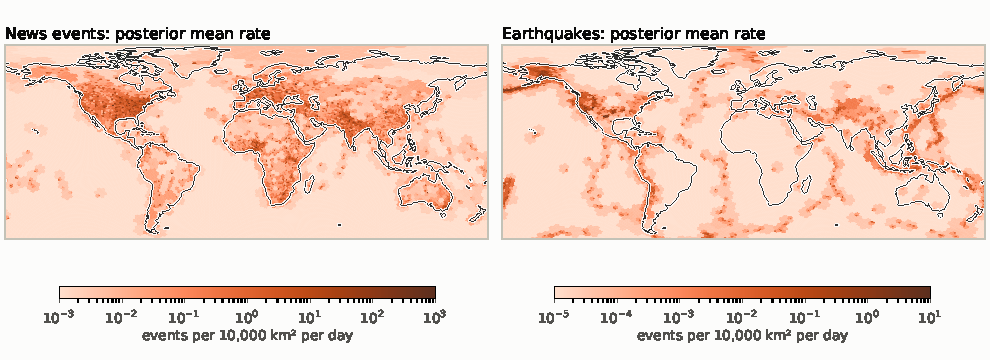
\includegraphics[width=\linewidth]{figures/globe_rates.pdf}
\caption{Posterior mean rate per cell, averaged over every partition of the tree.}
\label{fig:rates}
\end{figure}

\begin{table}[t]
\centering\small
\begin{tabular}{@{}lrrrrrr@{}}
\toprule
& \multicolumn{3}{c}{news events} & \multicolumn{3}{c}{earthquakes} \\
\cmidrule(lr){2-4}\cmidrule(l){5-7}
place & res. & area (km\textsuperscript{2}) & events & res. & area (km\textsuperscript{2}) & events \\
\midrule
\rows{data/places_table.tex}
\bottomrule
\end{tabular}
\caption{The bin of the best partition around a few places: its H3 resolution, area and number
of events.}
\label{tab:places}
\end{table}

\subsection{Held-out prediction}

Each dataset was split at the middle of its time span (news: \newsTrainDays\ days with
\newsTrainEvents\ events, then \newsTestDays\ days with \newsTestEvents; earthquakes:
\quakeTrainDays\ days with \quakeTrainEvents, then \quakeTestDays\ days with \quakeTestEvents). Every
method was fitted to the first half, with its prior chosen by its own training evidence, and scored
by $\log P(\text{test} \mid \text{train})$, the joint predictive of every cell's count in the second
half. For a fixed partition this is $\sum_B [\log L_B(\text{train}+\text{test}) - \log
L_B(\text{train})]$; for the tree averaged over its partitions it is $\log Z(\text{train}+\text{test})
- \log Z(\text{train})$, exactly, because the bins' rates are shared by both halves.

\Cref{tab:heldout,fig:heldout} give the results. The tree averaged over its partitions predicts best
for both. It beats the finest fixed grid, one rate per cell with no pooling, by \newsGainGrid\ nats
for news and \quakeGainGrid\ for earthquakes (\newsGainGridPerEvent\ and \quakeGainGridPerEvent\
nats per held-out event); coarser grids are far worse. The tree's single best partition comes close
(\newsBestPerEvent\ and \quakeBestPerEvent). Greedy merging predicts worse than the finest
grid (\newsMergedPerEvent\ and \quakeMergedPerEvent\ per event), and still does without its bonus
(\newsMergedNoBonusPerEvent\ and \quakeMergedNoBonusPerEvent); charging a cost per merge only
returns the tree's own best partition. The merged maps are for display; predictions should come
from the tree. All methods lose to the change in volume between the halves (\newsTestChange\ for
news), which no stationary model can anticipate.

The evidence is a sequential predictive score: for any order of the data, $\log P(D) = \sum_t \log
P(y_t \mid y_{<t})$ \citep{dawid1984present}. Choosing a prior by the evidence is choosing it by
prediction, and averaging over partitions is the best predictor under the model. The held-out test
checks this where the model is not exactly right.

\begin{table}[t]
\centering\small
\begin{tabular}{@{}lrrrr@{}}
\toprule
& \multicolumn{2}{c}{news events} & \multicolumn{2}{c}{earthquakes} \\
\cmidrule(lr){2-3}\cmidrule(l){4-5}
method & bins & nats/event & bins & nats/event \\
\midrule
\rows{data/heldout_table.tex}
\bottomrule
\end{tabular}
\caption{Held-out prediction of the second half of each record from the first: $\log
P(\text{test} \mid \text{train})$ per held-out event, relative to the best method (higher is
better). ``Bonus'' and ``cost'' are the per-merge terms of greedy merging.}
\label{tab:heldout}
\end{table}

\begin{figure}[t]
\centering
\pgfplotsset{heldout/.style={xbar, width=0.42\linewidth, height=4.2cm, bar width=7pt,
    ytick=data, tick label style={font=\scriptsize}, label style={font=\footnotesize},
    xlabel={nats per held-out event}, xmax=0.02, scaled x ticks=false,
    xticklabel style={/pgf/number format/fixed, /pgf/number format/precision=2}, enlarge y limits=0.15, axis x line*=bottom,
    axis y line*=left, xmajorgrids, grid style={gray!20}}}
\begin{tikzpicture}
\begin{axis}[heldout, title={\footnotesize news events}, yticklabels from table={data/plot_heldout_gdelt.csv}{label}, table/col sep=semicolon]
  \addplot[fill=binline, draw=none] table[col sep=semicolon, x=per_event, y expr=\coordindex] {data/plot_heldout_gdelt.csv};
\end{axis}
\end{tikzpicture}\hfill
\begin{tikzpicture}
\begin{axis}[heldout, title={\footnotesize earthquakes}, yticklabels={}]
  \addplot[fill=accent, draw=none] table[col sep=semicolon, x=per_event, y expr=\coordindex] {data/plot_heldout_usgs.csv};
\end{axis}
\end{tikzpicture}
\caption{The closest methods of \cref{tab:heldout}, relative to the tree averaged over its
partitions.}
\label{fig:heldout}
\end{figure}

\subsection{Does a hierarchy help in one dimension?}

In one dimension the original prior already sums over every segmentation, so a hierarchy can only
restrict or reweight it. A binary-cut tree (\cref{eq:guillotine} on an interval) builds the same
segmentations with a prior over cut trees, at $O(T^3)$; a dyadic tree allows boundaries only at
midpoints, at $O(T)$. On hourly world earthquake counts (\oneDT\ hours, \oneDEvents\ events; the
original prior's most probable $M$ is \oneDMmap), with the same Gamma prior per bin, the binary-cut
tree's evidence differs from the original prior's by \oneDBinaryGain\ nats, a tie, at
\oneDBinarySeconds\ per value of $\rho$ against \oneDBayesbinSeconds; the dyadic tree's is
\oneDDyadicLoss\ nats lower. A hierarchy helps one-dimensional data only through speed on very long
series, or where a second axis hides in the data: trial blocks $\times$ time for a response that
changes during a recording, or groups of days $\times$ time of day.

% ----------------------------------------------------------------------------------------------
\section{Three and more dimensions}\label{sec:higher}

Nesting stays quadratic in the number of cells in any dimension. With $d$ ordered axes, cut the
first into slabs, each slab's second axis into bands, and so on; each level is a 1-D recursion
whose bin evidences are the marginal likelihoods of the level below, and the cost is $O(M
\prod_i m_i^2) = O(MN^2)$ for $N = \prod_i m_i$ cells. Recursive cuts in $d$ dimensions have about
$N^2/2^d$ sub-boxes with $\sum_i m_i$ cuts each, so $O(N^2 \sum_i m_i)$ time and $N^2/2^d$ memory;
octrees and other dyadic hierarchies are linear in the number of nodes. Space--time binning is the
case Worldwatch needs: two dimensions of the sphere and one of time, which \cref{eq:blocks} makes
exact at $O(\text{nodes} \cdot T^3)$; with candidate time boundaries at the edges of a geometric
cascade of bins (about eight per octave of age), $T$ stays near a hundred over months. Product
grids and general partitions remain hard in every dimension.

% ----------------------------------------------------------------------------------------------
\section{Discussion}

The dynamic programme of Bayesian binning does not need an ordered axis, only partitions built from
sub-problems that meet at their boundaries. Nesting chains and trees keeps the exact sum and its
posteriors in two dimensions and more; sharing choices across the grid or allowing free shapes loses
it. Over the globe, a recursion over the H3 tree is cheap enough to choose its prior by the evidence
and gives bins of four million square kilometres over empty ocean and the finest cells where events
are, and its posterior average predicted held-out data better than any fixed grid.

Of the optimisations of the 1-D implementation, those inside each 1-D pass carry over unchanged to
rows then columns, which calls the 1-D code for every band: block-wise matrix products, fused
multi-threaded kernels, the handling of underflow and an exact fallback, and $O(MT)$ memory.
Prefix sums become summed-area tables. Batching the bands into one kernel is new work, and would
remove the call overhead that dominates at small sizes. The tree over H3 needs none of them; it is
cheap in plain log space. Recursive cuts gain nothing from them, since their table of inside values
is quadratic in the number of cells by nature and their sums run in order of rectangle size.

Several things limit the present results. The finest cells are those of the archive (resolution
\finestRes); finer data would give cities smaller bins at the same cost per node. A child without
events is taken as one empty bin. The records are short (\newsDays\ days of news), and their volume
changes over time, which stationary models cannot follow; the change-point models of
\cref{sec:spacetime} address that, and the burst factor of overdispersed counts can enter each
region's model. The pipeline that produces every number here reruns on new data
(\cref{app:repro}).

\bibliographystyle{plainnat}
\bibliography{refs}

\appendix
\section{Reproducing the numbers}\label{app:repro}

Every number in this draft is a macro written by \texttt{scripts/macros.py}, every table body and
plotted series a file in \texttt{data/}, and every map a figure drawn by \texttt{scripts/maps.py},
all from the pipeline in \texttt{scripts/}: \texttt{globe.py} (the tree over H3 on all the data),
\texttt{predict.py} (held-out prediction), \texttt{tree1d.py} (the 1-D comparison) and
\texttt{rectangles.py} (the rectangle families, their checks, counts and timings). \texttt{make data}
reruns it on the current data and \texttt{make} rebuilds this PDF. Qualitative claims in the text
are checked against the new results, and any that no longer hold are listed under the abstract.

\end{document}
